\documentclass{standalone}
\usepackage{tikz}
\usetikzlibrary{patterns, positioning}


\begin{document}
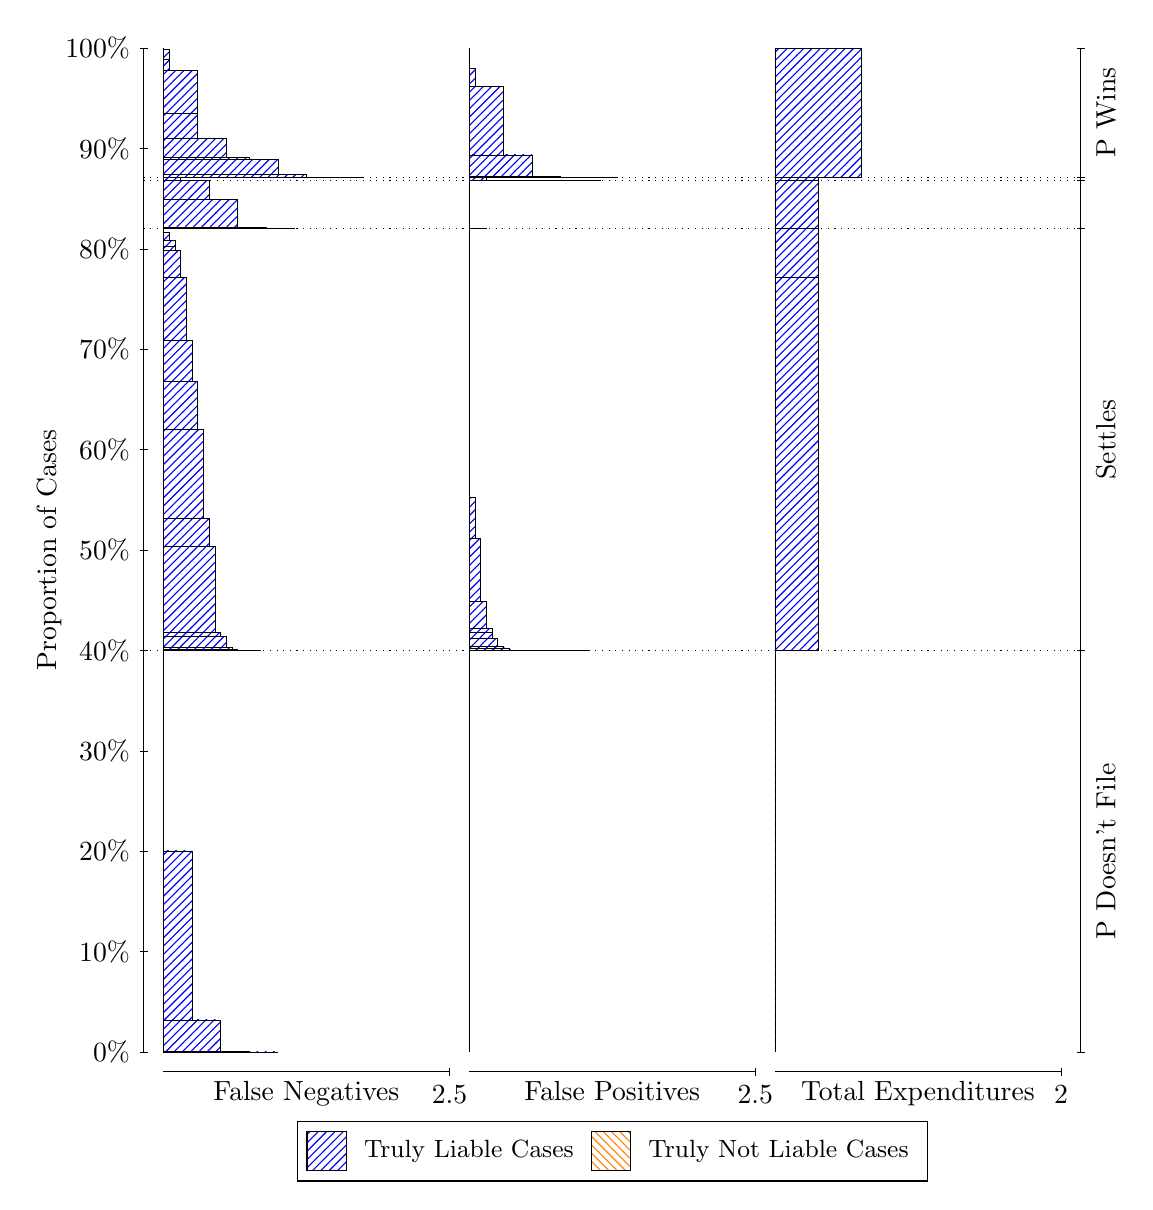
\begin{tikzpicture}
\draw[black, very thin] (1.5,1.75) -- (1.5,14.5);
\node[rotate=90, text=black, anchor=center] at (0.3, 8.125) {Proportion of Cases};
\draw[black, very thin] (1.45,1.75) -- (1.55,1.75);
\node[text=black, anchor=east] at (1.45, 1.75) {0\%};
\draw[black, very thin] (1.45,3.025) -- (1.55,3.025);
\node[text=black, anchor=east] at (1.45, 3.025) {10\%};
\draw[black, very thin] (1.45,4.3) -- (1.55,4.3);
\node[text=black, anchor=east] at (1.45, 4.3) {20\%};
\draw[black, very thin] (1.45,5.575) -- (1.55,5.575);
\node[text=black, anchor=east] at (1.45, 5.575) {30\%};
\draw[black, very thin] (1.45,6.85) -- (1.55,6.85);
\node[text=black, anchor=east] at (1.45, 6.85) {40\%};
\draw[black, very thin] (1.45,8.125) -- (1.55,8.125);
\node[text=black, anchor=east] at (1.45, 8.125) {50\%};
\draw[black, very thin] (1.45,9.4) -- (1.55,9.4);
\node[text=black, anchor=east] at (1.45, 9.4) {60\%};
\draw[black, very thin] (1.45,10.675) -- (1.55,10.675);
\node[text=black, anchor=east] at (1.45, 10.675) {70\%};
\draw[black, very thin] (1.45,11.95) -- (1.55,11.95);
\node[text=black, anchor=east] at (1.45, 11.95) {80\%};
\draw[black, very thin] (1.45,13.225) -- (1.55,13.225);
\node[text=black, anchor=east] at (1.45, 13.225) {90\%};
\draw[black, very thin] (1.45,14.5) -- (1.55,14.5);
\node[text=black, anchor=east] at (1.45, 14.5) {100\%};

\draw[black, very thin] (13.4,1.75) -- (13.4,14.5);
\draw[black, very thin] (13.35,1.75) -- (13.45,1.75);
\node[anchor=west] at (13.35, 1.75) {};
\draw[black, very thin] (13.35,6.8489) -- (13.45,6.8489);
\node[anchor=west] at (13.35, 6.8489) {};
\draw[black, very thin] (13.35,12.211) -- (13.45,12.211);
\node[anchor=west] at (13.35, 12.211) {};
\draw[black, very thin] (13.35,12.817) -- (13.45,12.817);
\node[anchor=west] at (13.35, 12.817) {};
\draw[black, very thin] (13.35,12.859) -- (13.45,12.859);
\node[anchor=west] at (13.35, 12.859) {};
\draw[black, very thin] (13.35,14.5) -- (13.45,14.5);
\node[anchor=west] at (13.35, 14.5) {};

\draw[black, very thin, pattern color=blue, pattern=north east lines] (1.75,1.75) rectangle (3.2033,1.75);
\draw[black, very thin, pattern color=blue, pattern=north east lines] (1.75,1.75) rectangle (2.84,1.7534);
\draw[black, very thin, pattern color=blue, pattern=north east lines] (1.75,1.7534) rectangle (2.4767,2.158);
\draw[black, very thin, pattern color=blue, pattern=north east lines] (1.75,2.158) rectangle (2.1133,4.3029);
\draw[black, very thin, pattern color=orange, pattern=north west lines] (1.75,4.3029) rectangle (1.75,4.3029);
\draw[black, very thin, pattern color=blue, pattern=north east lines] (1.75,4.3029) rectangle (1.75,6.8489);
\draw[black, very thin, pattern color=blue, pattern=north east lines] (1.75,6.8489) rectangle (2.9853,6.8489);
\draw[black, very thin, pattern color=blue, pattern=north east lines] (1.75,6.8489) rectangle (2.84,6.849);
\draw[black, very thin, pattern color=blue, pattern=north east lines] (1.75,6.849) rectangle (2.6947,6.8612);
\draw[black, very thin, pattern color=blue, pattern=north east lines] (1.75,6.8612) rectangle (2.622,6.8898);
\draw[black, very thin, pattern color=blue, pattern=north east lines] (1.75,6.8898) rectangle (2.5493,7.028);
\draw[black, very thin, pattern color=blue, pattern=north east lines] (1.75,7.028) rectangle (2.4767,7.0824);
\draw[black, very thin, pattern color=blue, pattern=north east lines] (1.75,7.0824) rectangle (2.404,8.1661);
\draw[black, very thin, pattern color=blue, pattern=north east lines] (1.75,8.1661) rectangle (2.3313,8.5285);
\draw[black, very thin, pattern color=blue, pattern=north east lines] (1.75,8.5285) rectangle (2.2587,9.6546);
\draw[black, very thin, pattern color=blue, pattern=north east lines] (1.75,9.6546) rectangle (2.186,10.271);
\draw[black, very thin, pattern color=blue, pattern=north east lines] (1.75,10.271) rectangle (2.1133,10.789);
\draw[black, very thin, pattern color=blue, pattern=north east lines] (1.75,10.789) rectangle (2.0407,11.591);
\draw[black, very thin, pattern color=blue, pattern=north east lines] (1.75,11.591) rectangle (1.968,11.932);
\draw[black, very thin, pattern color=blue, pattern=north east lines] (1.75,11.932) rectangle (1.8953,11.979);
\draw[black, very thin, pattern color=blue, pattern=north east lines] (1.75,11.979) rectangle (1.8953,12.058);
\draw[black, very thin, pattern color=blue, pattern=north east lines] (1.75,12.058) rectangle (1.8227,12.154);
\draw[black, very thin, pattern color=orange, pattern=north west lines] (1.75,12.154) rectangle (1.75,12.154);
\draw[black, very thin, pattern color=blue, pattern=north east lines] (1.75,12.154) rectangle (1.75,12.211);
\draw[black, very thin, pattern color=blue, pattern=north east lines] (1.75,12.211) rectangle (3.4213,12.211);
\draw[black, very thin, pattern color=blue, pattern=north east lines] (1.75,12.211) rectangle (3.058,12.221);
\draw[black, very thin, pattern color=blue, pattern=north east lines] (1.75,12.221) rectangle (2.6947,12.58);
\draw[black, very thin, pattern color=blue, pattern=north east lines] (1.75,12.58) rectangle (2.3313,12.815);
\draw[black, very thin, pattern color=blue, pattern=north east lines] (1.75,12.815) rectangle (1.968,12.817);
\draw[black, very thin, pattern color=orange, pattern=north west lines] (1.75,12.817) rectangle (1.75,12.817);
\draw[black, very thin, pattern color=blue, pattern=north east lines] (1.75,12.817) rectangle (1.968,12.854);
\draw[black, very thin, pattern color=orange, pattern=north west lines] (1.75,12.854) rectangle (1.75,12.854);
\draw[black, very thin, pattern color=blue, pattern=north east lines] (1.75,12.854) rectangle (1.75,12.859);
\draw[black, very thin, pattern color=blue, pattern=north east lines] (1.75,12.859) rectangle (4.2933,12.859);
\draw[black, very thin, pattern color=blue, pattern=north east lines] (1.75,12.859) rectangle (3.93,12.859);
\draw[black, very thin, pattern color=blue, pattern=north east lines] (1.75,12.859) rectangle (3.5667,12.897);
\draw[black, very thin, pattern color=blue, pattern=north east lines] (1.75,12.897) rectangle (3.276,12.897);
\draw[black, very thin, pattern color=blue, pattern=north east lines] (1.75,12.897) rectangle (3.2033,13.081);
\draw[black, very thin, pattern color=blue, pattern=north east lines] (1.75,13.081) rectangle (2.9127,13.082);
\draw[black, very thin, pattern color=blue, pattern=north east lines] (1.75,13.082) rectangle (2.84,13.114);
\draw[black, very thin, pattern color=blue, pattern=north east lines] (1.75,13.114) rectangle (2.5493,13.348);
\draw[black, very thin, pattern color=blue, pattern=north east lines] (1.75,13.348) rectangle (2.4767,13.348);
\draw[black, very thin, pattern color=blue, pattern=north east lines] (1.75,13.348) rectangle (2.186,13.667);
\draw[black, very thin, pattern color=blue, pattern=north east lines] (1.75,13.667) rectangle (2.186,14.217);
\draw[black, very thin, pattern color=blue, pattern=north east lines] (1.75,14.217) rectangle (2.1133,14.217);
\draw[black, very thin, pattern color=blue, pattern=north east lines] (1.75,14.217) rectangle (1.8227,14.353);
\draw[black, very thin, pattern color=blue, pattern=north east lines] (1.75,14.353) rectangle (1.8227,14.487);
\draw[black, very thin, pattern color=orange, pattern=north west lines] (1.75,14.487) rectangle (1.75,14.487);
\draw[black, very thin, pattern color=blue, pattern=north east lines] (1.75,14.487) rectangle (1.75,14.5);
\draw[black, very thin, pattern color=orange, pattern=north west lines] (5.6333,1.75) rectangle (5.6333,1.75);
\draw[black, very thin, pattern color=blue, pattern=north east lines] (5.6333,1.75) rectangle (5.6333,6.8489);
\draw[black, very thin, pattern color=orange, pattern=north west lines] (5.6333,6.8489) rectangle (7.1593,6.8489);
\draw[black, very thin, pattern color=blue, pattern=north east lines] (5.6333,6.8489) rectangle (7.1593,6.8489);
\draw[black, very thin, pattern color=orange, pattern=north west lines] (5.6333,6.8489) rectangle (7.014,6.8489);
\draw[black, very thin, pattern color=blue, pattern=north east lines] (5.6333,6.8489) rectangle (7.014,6.8489);
\draw[black, very thin, pattern color=orange, pattern=north west lines] (5.6333,6.8489) rectangle (6.8687,6.8489);
\draw[black, very thin, pattern color=blue, pattern=north east lines] (5.6333,6.8489) rectangle (6.8687,6.8489);
\draw[black, very thin, pattern color=blue, pattern=north east lines] (5.6333,6.8489) rectangle (6.796,6.8489);
\draw[black, very thin, pattern color=orange, pattern=north west lines] (5.6333,6.8489) rectangle (6.7233,6.8489);
\draw[black, very thin, pattern color=blue, pattern=north east lines] (5.6333,6.8489) rectangle (6.7233,6.8489);
\draw[black, very thin, pattern color=blue, pattern=north east lines] (5.6333,6.8489) rectangle (6.6507,6.8489);
\draw[black, very thin, pattern color=orange, pattern=north west lines] (5.6333,6.8489) rectangle (6.578,6.8489);
\draw[black, very thin, pattern color=blue, pattern=north east lines] (5.6333,6.8489) rectangle (6.578,6.8489);
\draw[black, very thin, pattern color=blue, pattern=north east lines] (5.6333,6.8489) rectangle (6.5053,6.8489);
\draw[black, very thin, pattern color=orange, pattern=north west lines] (5.6333,6.8489) rectangle (6.4327,6.8489);
\draw[black, very thin, pattern color=blue, pattern=north east lines] (5.6333,6.8489) rectangle (6.4327,6.8489);
\draw[black, very thin, pattern color=blue, pattern=north east lines] (5.6333,6.8489) rectangle (6.36,6.849);
\draw[black, very thin, pattern color=blue, pattern=north east lines] (5.6333,6.849) rectangle (6.2873,6.8491);
\draw[black, very thin, pattern color=orange, pattern=north west lines] (5.6333,6.8491) rectangle (6.2873,6.8491);
\draw[black, very thin, pattern color=blue, pattern=north east lines] (5.6333,6.8491) rectangle (6.2873,6.8492);
\draw[black, very thin, pattern color=blue, pattern=north east lines] (5.6333,6.8492) rectangle (6.2147,6.8565);
\draw[black, very thin, pattern color=blue, pattern=north east lines] (5.6333,6.8565) rectangle (6.142,6.8831);
\draw[black, very thin, pattern color=blue, pattern=north east lines] (5.6333,6.8831) rectangle (6.0693,6.9052);
\draw[black, very thin, pattern color=blue, pattern=north east lines] (5.6333,6.9052) rectangle (5.9967,7.0012);
\draw[black, very thin, pattern color=blue, pattern=north east lines] (5.6333,7.0012) rectangle (5.924,7.0806);
\draw[black, very thin, pattern color=blue, pattern=north east lines] (5.6333,7.0806) rectangle (5.924,7.1273);
\draw[black, very thin, pattern color=blue, pattern=north east lines] (5.6333,7.1273) rectangle (5.8513,7.4685);
\draw[black, very thin, pattern color=blue, pattern=north east lines] (5.6333,7.4685) rectangle (5.7787,8.2702);
\draw[black, very thin, pattern color=blue, pattern=north east lines] (5.6333,8.2702) rectangle (5.706,8.7891);
\draw[black, very thin, pattern color=blue, pattern=north east lines] (5.6333,8.7891) rectangle (5.6333,12.211);
\draw[black, very thin, pattern color=orange, pattern=north west lines] (5.6333,12.211) rectangle (5.8513,12.211);
\draw[black, very thin, pattern color=blue, pattern=north east lines] (5.6333,12.211) rectangle (5.8513,12.214);
\draw[black, very thin, pattern color=blue, pattern=north east lines] (5.6333,12.214) rectangle (5.6333,12.817);
\draw[black, very thin, pattern color=orange, pattern=north west lines] (5.6333,12.817) rectangle (7.3047,12.817);
\draw[black, very thin, pattern color=blue, pattern=north east lines] (5.6333,12.817) rectangle (7.3047,12.817);
\draw[black, very thin, pattern color=blue, pattern=north east lines] (5.6333,12.817) rectangle (6.9413,12.817);
\draw[black, very thin, pattern color=blue, pattern=north east lines] (5.6333,12.817) rectangle (6.578,12.817);
\draw[black, very thin, pattern color=blue, pattern=north east lines] (5.6333,12.817) rectangle (6.2147,12.822);
\draw[black, very thin, pattern color=blue, pattern=north east lines] (5.6333,12.822) rectangle (5.8513,12.859);
\draw[black, very thin, pattern color=orange, pattern=north west lines] (5.6333,12.859) rectangle (7.5227,12.859);
\draw[black, very thin, pattern color=blue, pattern=north east lines] (5.6333,12.859) rectangle (7.5227,12.859);
\draw[black, very thin, pattern color=orange, pattern=north west lines] (5.6333,12.859) rectangle (7.1593,12.859);
\draw[black, very thin, pattern color=blue, pattern=north east lines] (5.6333,12.859) rectangle (7.1593,12.859);
\draw[black, very thin, pattern color=orange, pattern=north west lines] (5.6333,12.859) rectangle (6.796,12.859);
\draw[black, very thin, pattern color=blue, pattern=north east lines] (5.6333,12.859) rectangle (6.796,12.872);
\draw[black, very thin, pattern color=orange, pattern=north west lines] (5.6333,12.872) rectangle (6.4327,12.872);
\draw[black, very thin, pattern color=blue, pattern=north east lines] (5.6333,12.872) rectangle (6.4327,13.142);
\draw[black, very thin, pattern color=orange, pattern=north west lines] (5.6333,13.142) rectangle (6.142,13.142);
\draw[black, very thin, pattern color=blue, pattern=north east lines] (5.6333,13.142) rectangle (6.142,13.142);
\draw[black, very thin, pattern color=blue, pattern=north east lines] (5.6333,13.142) rectangle (6.0693,14.011);
\draw[black, very thin, pattern color=orange, pattern=north west lines] (5.6333,14.011) rectangle (5.7787,14.011);
\draw[black, very thin, pattern color=blue, pattern=north east lines] (5.6333,14.011) rectangle (5.7787,14.011);
\draw[black, very thin, pattern color=blue, pattern=north east lines] (5.6333,14.011) rectangle (5.706,14.245);
\draw[black, very thin, pattern color=orange, pattern=north west lines] (5.6333,14.245) rectangle (5.6333,14.245);
\draw[black, very thin, pattern color=blue, pattern=north east lines] (5.6333,14.245) rectangle (5.6333,14.5);
\draw[black, very thin, pattern color=orange, pattern=north west lines] (9.5167,1.75) rectangle (9.5167,1.75);
\draw[black, very thin, pattern color=blue, pattern=north east lines] (9.5167,1.75) rectangle (9.5167,6.8489);
\draw[black, very thin, pattern color=orange, pattern=north west lines] (9.5167,6.8489) rectangle (10.062,6.8489);
\draw[black, very thin, pattern color=blue, pattern=north east lines] (9.5167,6.8489) rectangle (10.062,11.585);
\draw[black, very thin, pattern color=orange, pattern=north west lines] (9.5167,11.585) rectangle (10.062,11.585);
\draw[black, very thin, pattern color=blue, pattern=north east lines] (9.5167,11.585) rectangle (10.062,12.211);
\draw[black, very thin, pattern color=orange, pattern=north west lines] (9.5167,12.211) rectangle (10.062,12.211);
\draw[black, very thin, pattern color=blue, pattern=north east lines] (9.5167,12.211) rectangle (10.062,12.817);
\draw[black, very thin, pattern color=orange, pattern=north west lines] (9.5167,12.817) rectangle (10.062,12.817);
\draw[black, very thin, pattern color=blue, pattern=north east lines] (9.5167,12.817) rectangle (10.062,12.859);
\draw[black, very thin, pattern color=orange, pattern=north west lines] (9.5167,12.859) rectangle (10.607,12.859);
\draw[black, very thin, pattern color=blue, pattern=north east lines] (9.5167,12.859) rectangle (10.607,14.5);
\draw[black, dotted] (1.5,6.8489) -- (13.4,6.8489);
\draw[black, dotted] (1.5,12.211) -- (13.4,12.211);
\draw[black, dotted] (1.5,12.817) -- (13.4,12.817);
\draw[black, dotted] (1.5,12.859) -- (13.4,12.859);
\draw[black, very thin] (1.75,1.5) -- (5.3833,1.5);
\node[text=black, anchor=north] at (3.5667, 1.5) {False Negatives};
\draw[black, very thin] (5.3833,1.45) -- (5.3833,1.55);
\node[text=black, anchor=north] at (5.3833, 1.45) {2.5};

\draw[black, very thin] (5.6333,1.5) -- (9.2667,1.5);
\node[text=black, anchor=north] at (7.45, 1.5) {False Positives};
\draw[black, very thin] (9.2667,1.45) -- (9.2667,1.55);
\node[text=black, anchor=north] at (9.2667, 1.45) {2.5};

\draw[black, very thin] (9.5167,1.5) -- (13.15,1.5);
\node[text=black, anchor=north] at (11.333, 1.5) {Total Expenditures};
\draw[black, very thin] (13.15,1.45) -- (13.15,1.55);
\node[text=black, anchor=north] at (13.15, 1.45) {2};

\node[text=black, centered, rotate=90] at (13.72, 4.2994) {P Doesn't File};
\node[text=black, centered, rotate=90] at (13.72, 9.5298) {Settles};


\node[text=black, centered, rotate=90] at (13.72, 13.679) {P Wins};

\draw (7.449999999999999,1.5) node[draw=none] (baseCoordinate) {};
\begin{scope}[align=center]
        \matrix[scale=0.5, draw=black, below=0.5cm of baseCoordinate, nodes={draw}, column sep=0.1cm]{
            \node[rectangle, draw, minimum width=0.5cm, minimum height=0.5cm, pattern color=blue, pattern=north east lines] {}; &
            \node[draw=none, font=\small, text=black] (B) {Truly Liable Cases}; &
            \node[rectangle, draw, minimum width=0.5cm, minimum height=0.5cm, pattern color=orange, pattern=north west lines] {}; &
            \node[draw=none, font=\small, text=black] (B) {Truly Not Liable Cases}; \\
            };
\end{scope}

\end{tikzpicture}
\end{document}